\documentclass[12pt]{article}
\usepackage[english]{babel}
\usepackage{amsmath,amsthm}
\usepackage{amsfonts}
\usepackage{graphicx}
\newtheorem{thm}{Theorem}[section]
\newtheorem{cor}[thm]{Corollary}
\newtheorem{lem}[thm]{Lemma}
\newtheorem{prop}[thm]{Proposition}
\theoremstyle{definition}
\newtheorem{defn}[thm]{Definition}
\theoremstyle{remark}
\newtheorem{rem}[thm]{Remark}
\numberwithin{equation}{section}
\begin{document}
\title{Regression of KL Software Distribution   }
\author{KL Software Libraries}
\date{Wed Nov 21 14:11:00 2012
}
\maketitle
\textbf{ KL Libraryt unit test ouput.  This LaTex file and the associated diagrams 		are produced by the KL software libraries.}
\subsubsection{Random Number Generator }
The sample size generated for this run is 100000.

\newpage
uniform \begin{tabular}{|c|c|c|c|}  mean & variance & skewness & kurtosis \\  \hline
$\mu_1 = 0.500298$ & $\mu_2 = 0.0835259$ & $\mu_3 = 0.00338757$ & $\mu_4 =1.80113$ \\
\end{tabular}

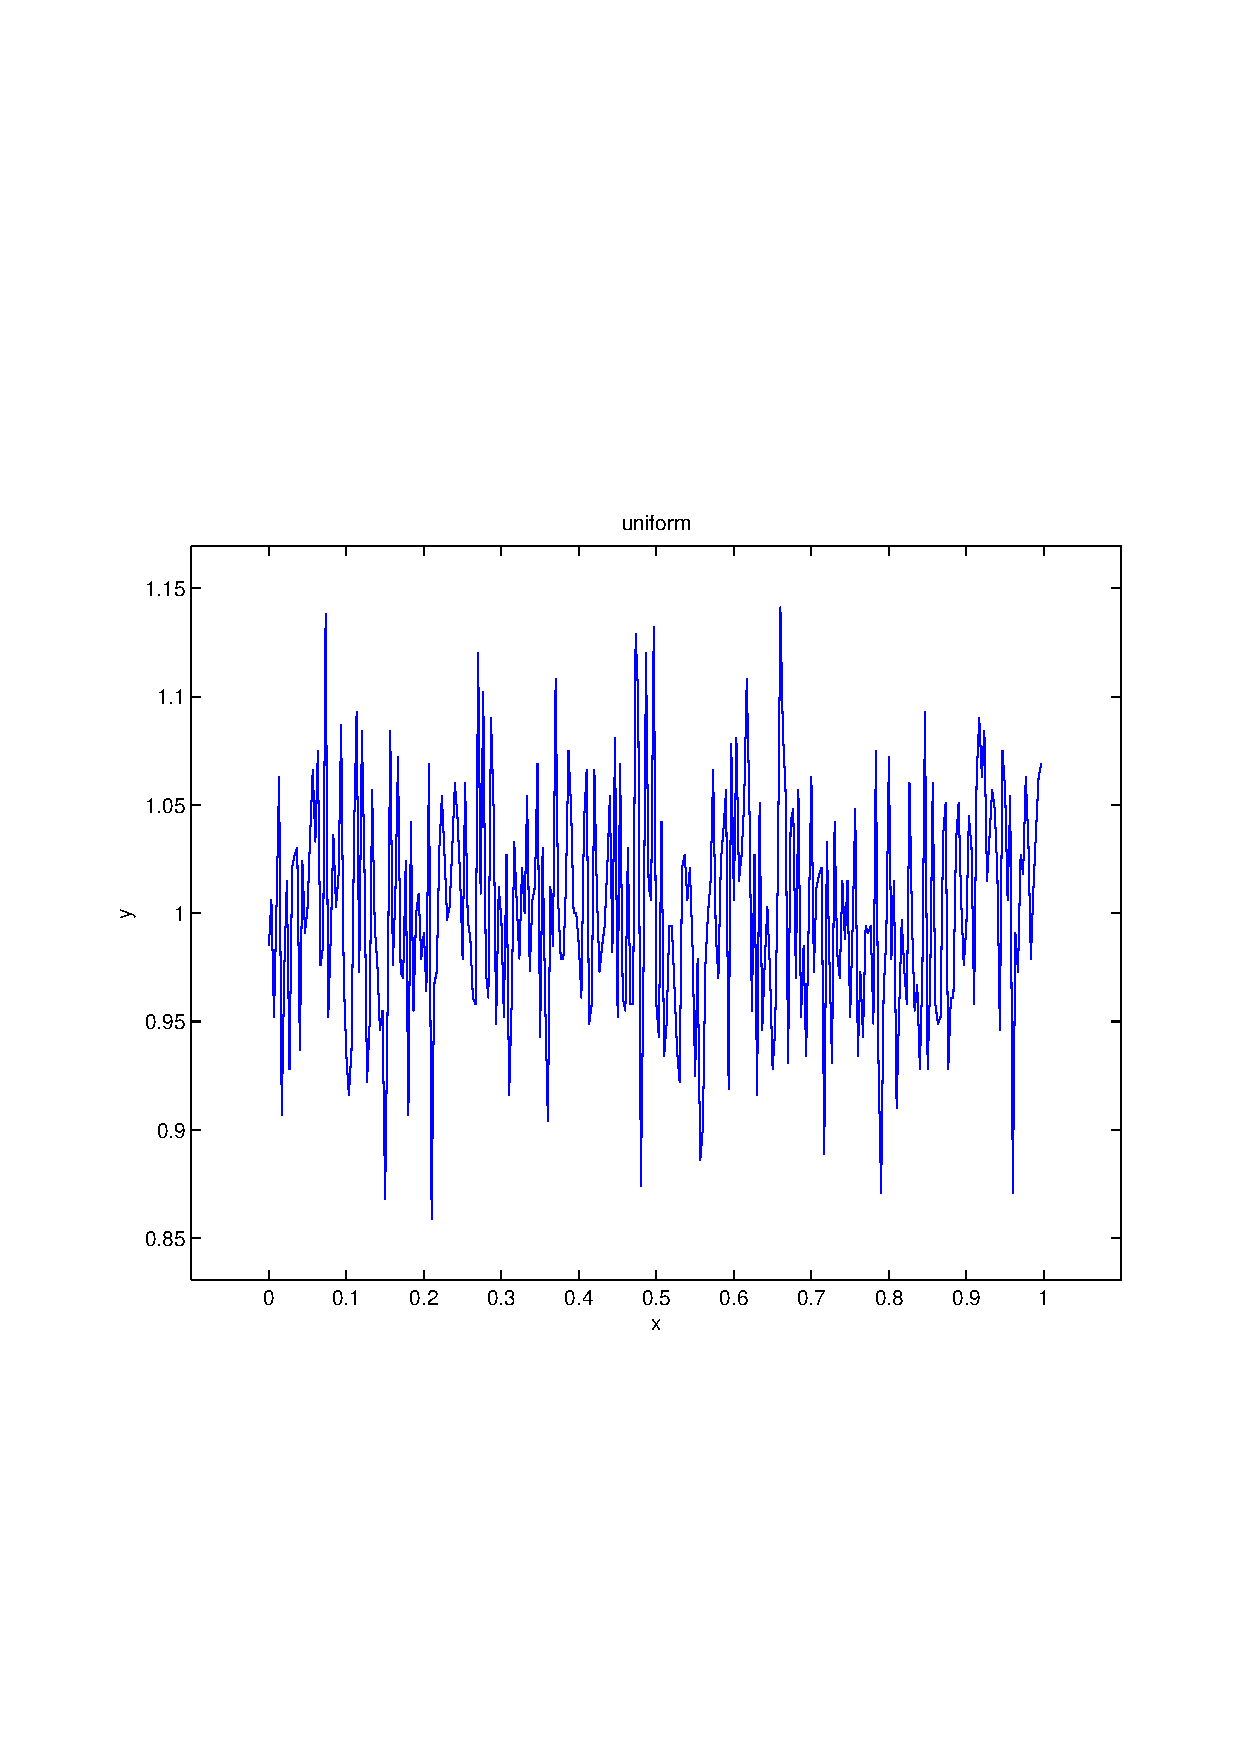
\includegraphics[width=5cm,height=5cm]{uniform.pdf}

cauchy \begin{tabular}{|c|c|c|c|}  mean & variance & skewness & kurtosis \\  \hline
$\mu_1 = 0.442883$ & $\mu_2 = 0.0534136$ & $\mu_3 = 0.63935$ & $\mu_4 =3.28094$ \\
\end{tabular}

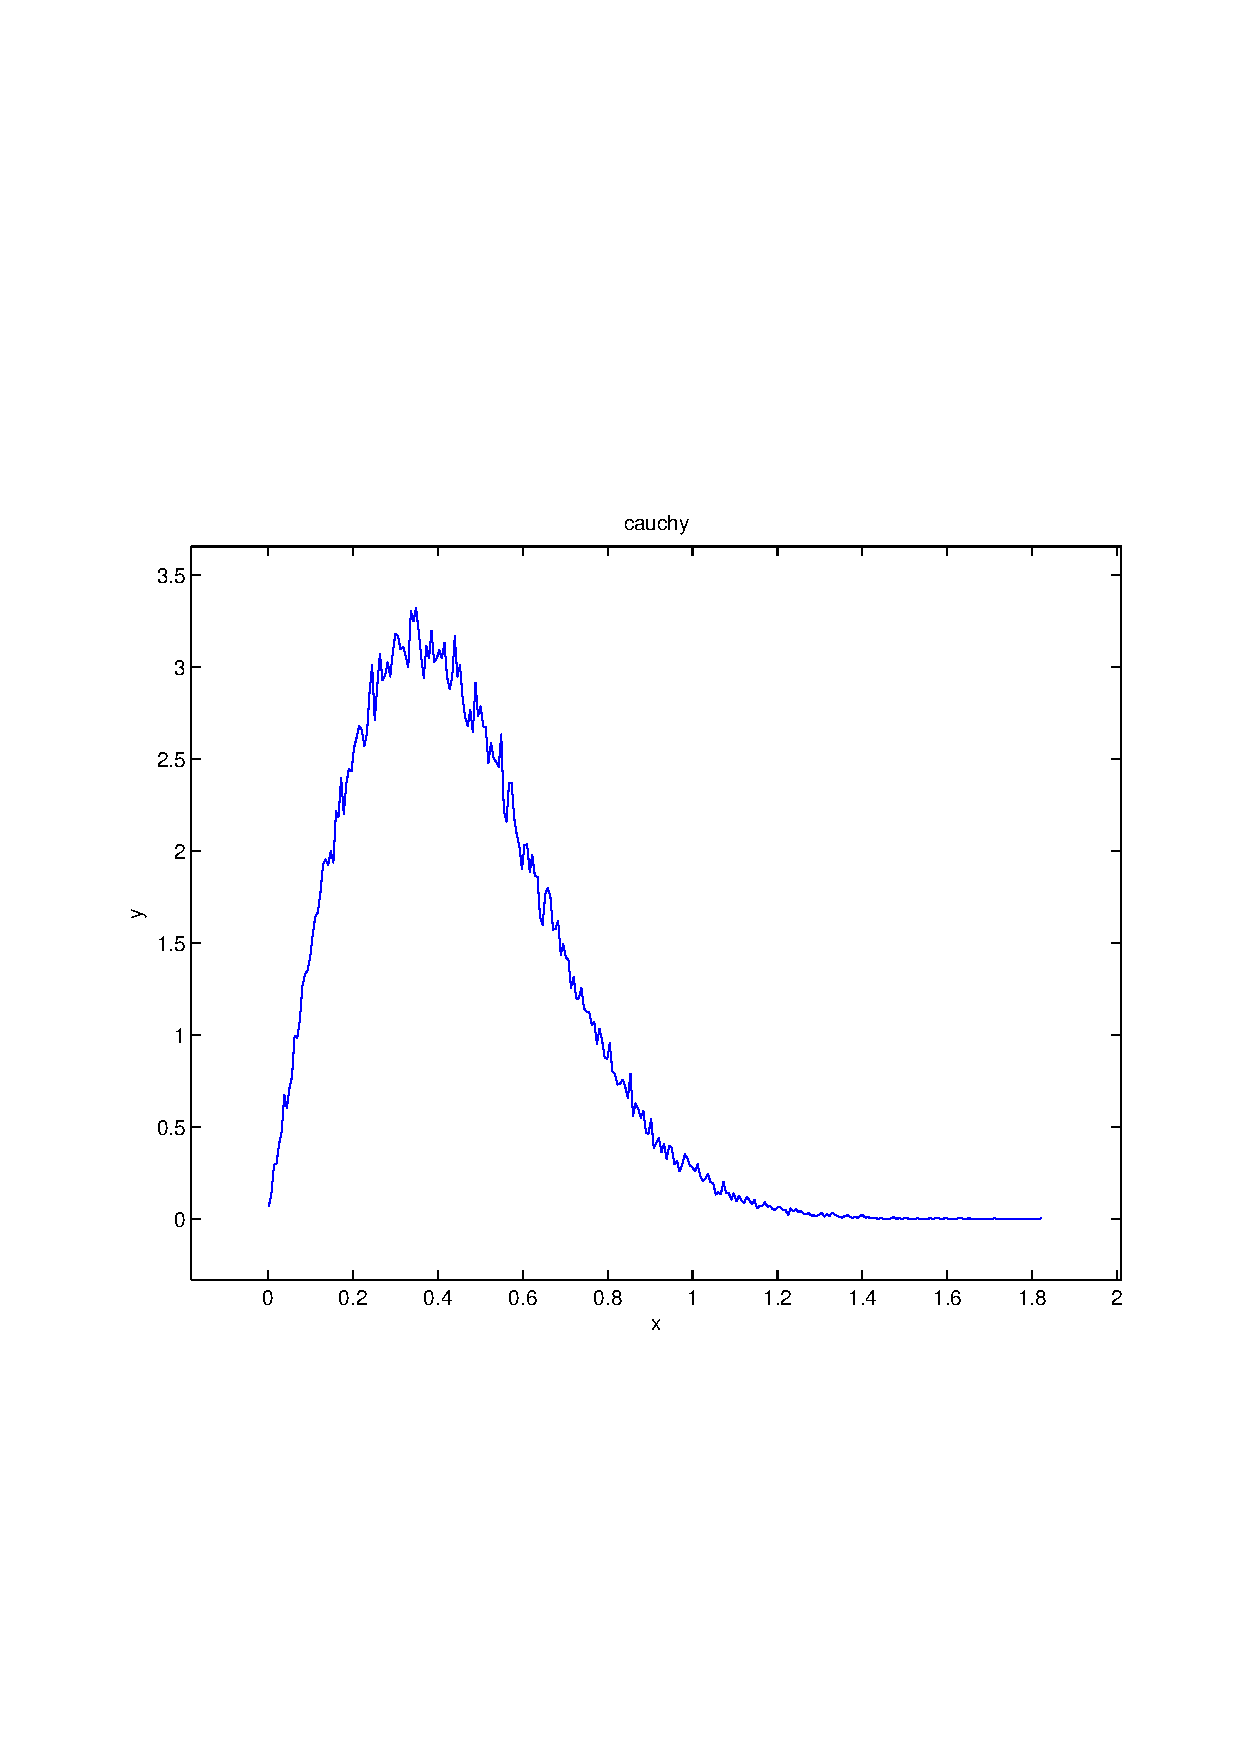
\includegraphics[width=5cm,height=5cm]{cauchy.pdf}

